\documentclass[11pt]{article}

\usepackage{amsmath}
\usepackage{amssymb}
\usepackage{subfigure}

\usepackage{pgfplots}
\usepackage{tikz}

% Available at (including additional examples):
% https://github.com/jluttine/tikz-bayesnet
\usetikzlibrary{bayesnet}

\begin{document}
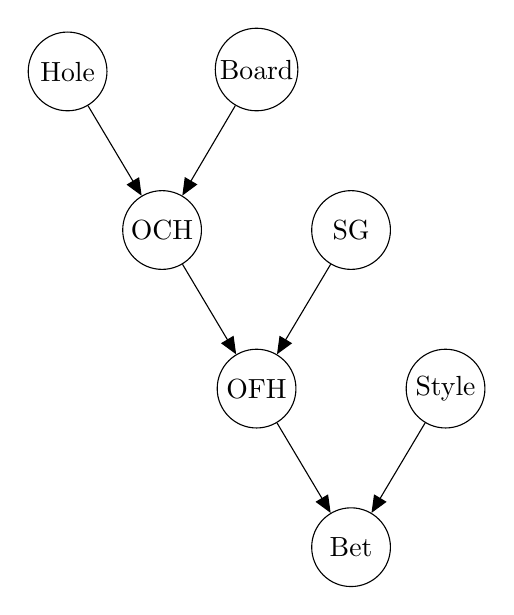
\begin{tikzpicture}
	% Define nodes
	\node[latent,minimum size=1cm] (bet) {Bet};
	\node[latent, above=of bet, xshift=-1.2cm,minimum size=1cm] (ofh) {OFH};
	\node[latent, above=of ofh, xshift=-1.2cm,minimum size=1cm] (och) {OCH};
	\node[latent, above=of ofh, xshift=1.2cm,minimum size=1cm] (sg) {SG};
	\node[latent, above=of och, xshift=1.2cm,minimum size=1cm] (board) {Board};
	\node[latent, above=of och, xshift=-1.2cm,minimum size=1cm] (hole) {Hole};
	\node[latent, above=of bet, xshift=1.2cm,minimum size=1cm] (style) {Style};
			
	% Connect the nodes
	\edge {style,ofh} {bet} ; %
	\edge {och,sg} {ofh} ; %
	\edge {hole,board} {och} ; %
\end{tikzpicture}
\end{document}